%% This document is created by 
%%  Dr. Putu Harry Gunawan
%% Template untuk Proposal TA 1 dan TA
%% Template ini digunakan untuk penulisan proposal TA 1 atau TA Fakultas Informatika, Telkom University.

\documentclass[a4paper,12pt,oneside]{book}
\usepackage[utf8]{inputenc}
\usepackage{sectsty}
\usepackage{graphicx}
\usepackage{epstopdf}
\usepackage{algorithm}
\usepackage{algpseudocode}
\usepackage{array}
\usepackage[table]{xcolor}
\usepackage{anysize}
\usepackage{amsmath}
\usepackage{amssymb}
\usepackage[bahasa]{babel}
\usepackage{indentfirst} %Spasi untuk paragraf pertama
\usepackage{geometry}
\usepackage{multirow}% http://ctan.org/pkg/multirow
\usepackage{hhline}% http://ctan.org/pkg/hhline
\marginsize{4cm}{3cm}{2cm}{3cm} %{left}{right}{top}{bottom}
\usepackage[compact]{titlesec} 
\usepackage{etoolbox}

\makeatletter
\patchcmd{\ttlh@hang}{\parindent\z@}{\parindent\z@\leavevmode}{}{}
\patchcmd{\ttlh@hang}{\noindent}{}{}{}
\makeatother

\chapterfont{\centering}
\newcommand{\bigsize}{\fontsize{16pt}{14pt}\selectfont}
\chapterfont{\centering\bigsize\bfseries}
\sectionfont{\large\bfseries}
\usepackage{tikz}
\usetikzlibrary{shapes.geometric, arrows}
%\renewcommand{\chaptertitle}{BAB}
\renewcommand{\thechapter}{\Roman{chapter}}
\renewcommand\thesection{\arabic{chapter}.\arabic{section}}
\renewcommand\thesubsection{\thesection.\arabic{subsection}}
\renewcommand{\theequation}{\arabic{chapter}.\arabic{equation}}
\renewcommand{\thefigure}{\arabic{chapter}.\arabic{figure}}
\renewcommand{\thetable}{\arabic{chapter}.\arabic{table}}
%\renewcommand*{\chapterheadstartvskip}{\vspace*{-\topskip}}

\usepackage{titlesec}

\titleformat{\chapter}[display]
{\centering\normalfont\bigsize\bfseries}{\chaptertitlename\ \thechapter}{20pt}{\bigsize}
\titlespacing*{\chapter}{0pt}{0pt}{40pt}


\renewcommand\bibname{Daftar Pustaka}
\addto{\captionsbahasa}{\renewcommand{\bibname}{Daftar Pustaka}}
\usepackage{fancyhdr}
\pagestyle{fancy}
\lhead{}
\chead{}
\rhead{}
\lfoot{}
\cfoot{\thepage}
\rfoot{}
\renewcommand{\headrulewidth}{0pt}

\makeatletter

%%%%%%%%%%%%%%%%%%%%%%%%%%%%%%%%%%%%%%%%%%%%%%%%%%%%%%%%%%%%
%
%  Berikut adalah data-data yang wajib diisi oleh mahasiswa
%
%%%%%%%%%%%%%%%%%%%%%%%%%%%%%%%%%%%%%%%%%%%%%%%%%%%%%%%%%%%%

\title{Analisis dan Implementasi Algoritma Rete untuk Sistem Pakar Pemilihan Unit Gawat Darurat di Kota Bandung}\let\Title\@title   %Judul dalam bahasa Indonesia

\newcommand{\EngTitle}{Analysis and Implementation of Expert System using Rete Algorithm for Selecting Emergency Room in Bandung City}  %Judul dalam bahasa Inggris

\author{Aji Tri Santoso}  \let\Author\@author  %Nama mhs
\newcommand{\NIM}{1103120130}
\newcommand{\Prodi}{Teknik Informatika}
\newcommand{\KK}{SIDE}
\newcommand{\Gelar}{Komputer} 
\date{2016}           \let\Date\@date %Maskkan hanya tahun saja
\newcommand{\Tanggal}{22} % Tanggal Pengesahan
\newcommand{\Bulan}{Agustus} % Bulan Pengesahan
\newcommand{\PembimbingSatu}{Danang Junaedi, S.T., M.T.}
\newcommand{\NIPPembimbingSatu}{14781566}
\newcommand{\PembimbingDua}{Amarilis Putri Yanuarifiani, S.T., M.T.I.}
\newcommand{\NIPPembimbingDua}{14891266}
\newcommand{\Kaprodi}{Dr. Moch Arif Bijaksana, S.T., M.Sc}
\newcommand{\NIPKaprodi}{03650312-4}
\newif\iflogTA
\logTAtrue   %%%%%% WARNING kode ini diaktifkan untuk format TUGAS AKHIR
\makeatother
\linespread{1}


\begin{document}
\pagenumbering{roman} 
%%\maketitle
\begin{titlepage}
\thispagestyle{empty}
%\vspace*{0.7cm}
{\centering
\large
{\bigsize\bf \Title}\\
\vspace{ 0.5cm}
{\bigsize\bf \textsl \EngTitle}\\
\vspace{ 1cm}
\rm
\textbf{Tugas Akhir}\\
\vspace{0.5 cm}
Diajukan untuk memenuhi sebagian dari syarat
untuk memperoleh gelar Sarjana Komputer
Fakultas Informatika
TelkomUniversity
\vspace{0.5 cm}

\vspace{0.5 cm}
\textbf{\Author}\\ \textbf{NIM: \NIM}\\ 

\vspace{1 cm}

\begin{figure}[h]
{\centering {
\includegraphics[scale=0.17]{Tel-U-Logo.png}}\par}
\end{figure}

\vspace{1 cm}
{\bigsize\textbf{Program Studi Sarjana \Prodi}\\
\vspace{0.25 cm}
\textbf{Fakultas Informatika}\\
\vspace{0.5 cm}
\textbf{Universitas Telkom}\\
\vspace{0.5 cm}
\textbf{Bandung}\\
\vspace{0.5 cm}
\textbf{\Date}\\}
}
\pagebreak



\thispagestyle{empty}
\addcontentsline{toc}{chapter}{Lembar Persetujuan}
\begin{flushright}
	
\end{flushright}{\centering
\iflogTA
\textbf{\large Lembar Pengesahan}\\  %UNTUK TA
\else
\textbf{\large Lembar Persetujuan}\\
\fi
\vspace{0.5cm}
\textbf{\Title}\\
\vspace{0.5cm}
\textbf{\textsl{\EngTitle}}\\
\vspace{0.5cm}
\textbf{\Author}\\
\textbf{NIM: \NIM}\\
\vspace{1cm}

\iflogTA 
{ Tugas Akhir ini diterima dan disahkan untuk memenuhi sebagian dari syarat untuk memperoleh gelar sarjana \Gelar\\ Program Studi Sarjana \Prodi\\ Fakultas Informatika Universitas Telkom}\\  %% UNTUK TA
\else
{ Proposal ini diajukan sebagai usulan pembuatan tugas akhir pada\\ Program Studi Sarjana \Prodi\\ Fakultas Informatika Universitas Telkom}\\
\fi
\vspace{0.5cm}

{Bandung, \Tanggal\quad \Bulan \quad \Date}\\
{Menyetujui}\\

\vspace{0.5cm}
\iflogTA
\begin{center}
\begin{tabular}{  m{8cm}  m{8cm} }
Pembimbing 1 & Pembimbing 2
\end{tabular}
\end{center}
\else
\begin{center}
\begin{tabular}{  m{8cm}  m{8cm} }
Calon Pembimbing 1 & Calon Pembimbing 2
\end{tabular}
\end{center}
\fi
\begin{center}
\vspace{2cm}
\begin{tabular}{  m{8cm}  m{8cm} }
\underline{\PembimbingSatu} & \underline{\PembimbingDua} \\ 
NIP: \NIPPembimbingSatu & NIP: \NIPPembimbingDua
\end{tabular}
\end{center}
\vspace{0.5cm}
\iflogTA
Mengesahkan,\\   %% UNTUK TA
Kepala Program Studi \Prodi\\ %% UNTUK TA
\vspace{2.5cm}   %% UNTUK TA
\underline{\Kaprodi}\\ NIP: \NIPKaprodi\\  %% UNTUK TA
\fi
}
\pagebreak

\thispagestyle{empty}
\addcontentsline{toc}{chapter}{Lembar Pernyataan}
{\centering
\textbf{\large Lembar Pernyataan}\\
\vspace{1 cm}

}
Dengan ini saya menyatakan bahwa Tugas Akhir dengan judul “Analisis dan Implementasi Algoritma Rete untuk Sistem Pakar Pemilihan Unit Gawat Darurat di Kota Bandung” beserta seluruh isinya adalah benar-benar karya saya sendiri dan saya tidak melakukan penjiplakan atau pengutipan dengan cara-cara yang tidak sesuai dengan etika keilmuan ang berlaku dalam masyarakat keilmuan. Atas pernyataan ini, saya siap menanggung akibat yang dijatuhkan kepada saya apabila kemudian ditemukan adanya pelanggaran terhadap etika keilmuan dalam karya saya ini, atau ada klaim dari pihak lain terhadap keaslian karya ini.
\vspace{1 cm}

\setlength{\parindent}{45ex}
{Bandung, \Tanggal\quad \Bulan \quad \Date}\\

\setlength{\parindent}{45ex}
Yang membuat pernyataan\\
	
\vspace{1.25 cm}
\setlength{\parindent}{45ex}
Aji Tri Santoso\\
	




\pagebreak
\end{titlepage}
\addcontentsline{toc}{chapter}{Lembar Persembahan}
{\centering
	\textbf{\large Lembar Persembahan}\\
	\vspace{1cm}
}

Alhamdulillahirabbil ‘aalamin, Segala puji dan syukur bagi Allah, yang dengan nama-Nya bumi dihamparkan, yang dengan nama-Nya langit ditinggikan.  Kedamaian dan kesejahteraan dari-Nya semoga tercurah bagi Rasulullah saw, beserta keluarga, sahabat dan pengikutnya. Atas berkat rahmat Allah Subhanahu wa Taala, Ar-Rahman, Sang Maha Pengasih akhirnya penulis dapat menyelesaikan penulisan buku Tugas Akhir ini. Selama proses pengerjaan Tugas Akhir ini, penulis mendapat berbagai bimbingan dan wejangan dari berbagai macam pihak. Oleh karena itu, melalui Lembar Persembahan ini penulis mengucapkan rasa terimakasih kepada:

\begin{enumerate}
	\item Persembahan kasih kepada kedua Ibu, yang di Surga dan di Bumi, dan pernyataan bakti kepada Bapak.
	\item Kedua kakak tercinta, yang menjadi pegangan hidup dan panutan penulis.
	\item Bapak Danang Junaedi, M.T. yang membimbing penulis selama pengerjaan tugas akhir. Berbagi nilai-nilai kebenaran dan senantiasa bekerjasama dengan penulis, saya pribadi berharap dapat saling berbagi ilmu lagi di lain kesempatan.
	\item Seluruh keluarga IF 36 06 yang menemani hari-hari penulis, sampai bertemu di kesempatan lain.
	\item Seluruh civitas akademika Telkom University yang telah membangun karakter penulis dan menjadi tempat penulis mencari ilmu khususnya fakultas Informatika, 
	\item Seluruh anggota UKM jurnalistik Aksara Telkom University, telah menjadi rumah kedua penulis.
\end{enumerate}


\pagebreak

\addcontentsline{toc}{chapter}{Abstrak}
{\centering
	\textbf{\large Abstrak}\\
	\vspace{0.5cm}
}

%\chapter*{Abstrak}
Kejadian gawat darurat adalah kondisi dimana respon dibutuhkan dari pasien, keluarga, atau siapapun yang dianggap mempunyai kewajiban untuk mengambil keputusan membawa pasien ke rumah sakit untuk tindakan medis segera mungkin. Dalam menentukan pemilihan Unit Gawat Darurat (UGD) rumah sakit tujuan harus mempertimbangkan beberapa kriteria. Pada penelitian ini dibangun sistem pakar untuk mendapatkan kesesuaian UGD. Kriteria yang menjadi pertimbangan pemilihan UGD adalah kondisi pasien, waktu tempuh, ketersediaan dokter jaga, ketersediaan ruang operasi, ada ruang inap dan ruang ICU rumah sakit. Sistem pakar yang diabangun atas model berbasis pengetahuan (knowledge base). Pengetahuan yang disimpan menjadi rule diolah dengan mesin inferensi menggunakan algoritma Rete. Implementasi algoritma Rete yaitu dengan membuat hubungan antar node pada graf asiklik yang membentuk suatu jaringan Rete. Hubungan antar node dirancang agar bisa menghilangkan redundansi proses komputasi dari satu siklus ke siklus selanjutnya. Melalui penggunaan algoritma Rete pada rule based system diperoleh kecepatan dan efisiensi komputasi dengan mengurangi usaha yang dilakukan untuk komputasi berulang dari conflict set setelah aturan (rule) dieksekusi.
  
\vspace{0.5 cm}
\begin{flushleft}
{\textbf{Kata Kunci:} sistem pakar, algoritma Rete, knowledge base, inference engine, unit gawat darurat}
\end{flushleft}
\iflogTA
\pagebreak

\addcontentsline{toc}{chapter}{Abstract}
{\centering
	\textbf{\large Abstract}\\
	\vspace{0.5cm}
}

%\chapter*{Abstract}
  Emergency medical situation are conditions in which a rapid response is required from patient itself, family, or anyone nearby. In case of Emergency everyone is deemed to have obligation to make quick decision taking the patient to hospital for medical treatment. Transporting severely injured patients in emergency case can by time consuming and resource consuming. This practical application of our system can be used to determining suitable hospital for patient in timely manner.  Several objective and criteria should be considered to increase the patient’s life expectancy. In this study, we build Expert System (ES) to obtain suitable hospital using criteria patient conditions, travel time, availability of doctor, availability of operating room, ICU, and ICCU rooms. An Expert System built upon knowledge base model, this knowledge stored into rule and processed by inference engine using Rete Algorithm which is built from Rete network. The relationship in between nodes in Rete Algorithm designed to eliminate redundancy of computer processes of Expert System. Through the using of the Rete algorithm on the rule based system, the speed and efficiency of computing by reducing the effort made for repeated computation of the conflict set after the rule is executed.

\vspace{0.5 cm}
\begin{flushleft}
{\textbf{Keywords:} :  rete algorithm, expert system, inference engine, knowledge based.}
\end{flushleft}
\pagebreak

\addcontentsline{toc}{chapter}{Kata Pengantar}
{\centering
	\textbf{\large Kata Pengantar}\\
	\vspace{0.5cm}
}


%\chapter*{Kata Pengantar}
\begin{center}
\textsl{	Bismillahirrahmanirrahim.\\
	“Demi matahari dan cahayanya,\\
	dan bulan apabila mengiringinya,\\
	dan siang apabila menampakannya,\\
	dan malam apabila menutupinya.\\
	Dan langit serta yang membangunkannya.\\
	Dan bumi serta yang membentangkannya.\\
	Dan jiwa serta yang menyempurnakannya.” \\
	QS. Asy-Syams (Matahari) 91:1-7 }

\end{center}

Segala puji dan syukur bagi Allah semata, karena berkat rahmat dan kebesaran-Nya penulis dapat menyelesaikan penulisan buku Tugas Akhir dengan judul “Analisis dan Implementasi Algoritma Rete untuk Sistem Pakar Pemilihan Unit Gawat Darurat di Kota Bandung” sebagai salah satu syarat kelulusan pada Program Studi Teknik Informatika Universitas Telkom.
Akhirnya, penulis berharap penelitian ini mendapatkan sambutan yang baik dari masyarakat keilmuan dan memberi dampak yang bermanfaat pula bagi perubahan. Atas segala masukan, saran dan kritik demi perbaikan, penulis mengucapkan terimakasih.
Semoga Allah SWT senantiasa memudahkan dan melapangkan upaya kita dalam menjalankan Program-Nya. Amin.
\vspace{1.25 cm}
\begin{flushright}
	{Bandung, \Tanggal\quad \Bulan \quad \Date}\\
	\vspace{1.25 cm}
	Aji Tri Santoso\\
	
\end{flushright}

\pagebreak

\fi
\cleardoublepage

\addcontentsline{toc}{chapter}{Daftar Isi}
\tableofcontents
\iflogTA
\newpage
\cleardoublepage
\addcontentsline{toc}{chapter}{Daftar Gambar}
\listoffigures
\newpage
\cleardoublepage
\addcontentsline{toc}{chapter}{Daftar Tabel}
\listoftables
%\pagebreak
\fi
%
\cleardoublepage
\pagenumbering{arabic}

\chapter{Pendahuluan}
\section{Latar Belakang}
Kejadian gawat darurat dapat diartikan sebagai keadaan dimana seseorang membutuhkan pertolongan segera karena apabila tidak mendapatkan pertolongan dapat mengancam jiwa atau menimbulkan kecacatan. Menurut American Hospital Association (AHA) dalam Herkutanto \cite{herkutanto2007} keadaan darurat adalah kondisi dimana respon dibutuhkan dari pasien, keluarga, atau siapapun yang dianggap mempunyai kewajiban untuk mengambil keputusan membawa pasien ke rumah sakit untuk tindakan medis segera mungkin. Dalam penanganan gawat darurat fase pra-rumah sakit terlibat pula unsur-unsur masyarakat non-tenaga kesehatan. Kecepatan dan ketepatan tindakan pada fase pra-rumah sakit sangat menentukan tingkat keselamatan pasien.
Fase pra-rumah sakit dimulai ketika warga sekitar lokasi kejadi memberikan pertolongan pertama atau memanggil tim medis gawat darurat hingga selama transportasi ke rumah sakit. Pada fase ini waktu menjadi faktor penting berhubungan dengan tingkat keselamatan jiwa korban \cite{boswick}. Tidak setiap rumah sakit dapat menyediakan perawatan yang tepat sesuai kondisi korban pada saat kejadian gawat darurat. Kesalahan dalam membawa korban ke rumah sakit yang tidak sesuai kondisi korban dan sumber daya rumah sakit bisa berakibat mesti berpindahnya pasien ke tempat lain hingga menemukan kesesuaian. Pembuat keputusan harus menentukan secara tepat dan cepat pemilihan Unit Gawat Darurat (UGD) di rumah sakit tujuan. Sedangkan pembuat keputusan mungkin merupakan masyarakat awam di lokasi yang minim informasi penanganan gawat darurat. Untuk itu diperlukan sebuah sistem pakar untuk permasalahan pemilihan UGD
Kejadian yang sering terjadi adalah pengambil keputusan hanya memperhitungkan jarak rumah sakit terdekat. Padahal jika rumah sakit yang dituju tidak mempunyai ketersediaan dokter jaga sesuai kondisi korban, ketersediaan ruang ICU, ketersediaan ruang operasi maka harus berpindah ke rumah sakit lain hingga menemukan kesesuaian \cite{weng2009}. Sebagai contoh adalah pengalaman pribadi netizen yang termuat di portal berita \cite{priyono2015} yang ditolak dua rumah sakit dengan alasan kamar perawatan penuh dan tidak tersedia alat sesuai untuk menangani kondisi gawat darurat yang sedang dialami.
Weng dan Kuo \cite{weng2009} dalam penelitiannya membangun sistem pakar gawat darurat untuk daerah dengan sumber daya medis yang kurang. Dalam penelitannya Weng dan Kuo membuat knowledge base pemilihan UGD untuk menemukan kesesuaian antara UGD dan pasien. Mesin inferensi yang digunakan adalah metode runut maju (Forward Chaining). Priyandari \cite{priyandari2011} menggunakan model kaidah pemilihan UGD dari penelitian Weng dan Kuo tetapi mengganti kriteria jarak dengan estimasi waktu tempuh untuk mengatasi arus lalu lintas perkotaan yang padat. Mesin inferensi yang digunakan sama yaitu forward chaining. Dalam penerapan Forward chaining timbul masalah ketika rule-base terlalu besar karena terjadi repetisi pemeriksaan setiap rule
terhadap fakta akan mahal dari segi komputasi.Sehingga kompleksitas yang dihasilkan eksponensial \cite{freeman}.
Pada tugas akhir ini metode yang diusulkan untuk menentukan pemilihan UGD menggunakan algoritma Rete. Algoritma yang dikembangkan Dr. Charles Forgy \cite{charles1982} ini menggunakan hubungan antar nodes dalam graf asiklik berarah. Algoritma ini dipilih karena dapat memberikan peningkatan kecepatan komputasi forward chaining rule-based system dengan mengurangi usaha yang dilakukan untuk komputasi berulang dari conflict set setelah aturan (rule) dieksekusi. Faktor yang menjadi pertimbangan pemilihan adalah kondisi pasien, waktu tempuh lokasi ke UGD, ketersediaan dokter jaga, ketersediaan ruang operasi, ruang inap dan ruang ICU rumah sakit. Daerah kajian yang akan digunakan pada tugas akhir ini adalah rumah sakit dengan Unit Gawat Darurat di wilayah administrasi kota Bandung.
\section{Perumusan Masalah}
Berdasarkan latar belakang dirumuskan permasalahan sebagai berikut:
\begin{enumerate}
    \item Bagaimana implementasi algoritma Rete dalam memberikan pemilihan UGD?
    \item Bagaimana pengaruh penerapan algoritma Rete dalam sistem pakar pemilihan UGD?
    \item Bagaimana performansi sistem pakar dalam menghasilkan pemilihan UGD?
\end{enumerate}
\section{Batasan Masalah}
Adapun batasan masalah pada tugas akhir ini, yaitu:
\begin{enumerate}
	\item Perhitungan waktu tempuh dari titik lokasi kejadian gawat darurat ke UGD sudah diketahui dan tidak menjadi pokok bahasan.
	\item Rute yang dipilih untuk menuju UGD tidak menjadi pokok bahasan dalam tugas akhir ini.
\end{enumerate}
\section{Tujuan}
Tujuan dari dari tugas akhir ini antara lain:
\begin{enumerate}
    \item Mengetahui penerapan algoritma Rete hingga menghasilkan sistem pakar pemilihan UGD.
    \item Mengetahui pengaruh penerapan algoritma Rete dalam sistem pakar pemilihan UGD.
    \item Mengetahui pengaruh penerapan algoritma Rete dalam sistem pakar pemilihan UGD.
\end{enumerate}
\section{Metodelogi Penyelesaiaan Masalah}
Adapun metode penyelesaiaan yang akan dilakukan untuk penyelesaiaan tugas akhir ini yaitu:
\begin{enumerate}
	\item Studi Literatur\\
	Penulis melakukan pencarian informasi yang dibutuhkan untuk penyelesaiaan tugas akhir ini melalui buku, jurnal yang telah terindek publikasi, dan berbagai sumber lain yang membahas sistem pakar (expert system) serta algoritma Rete sehingga dapat merumuskan latar belakang dan kontribusi keilmuan dari penelitian yang dilakukan.
	\item Pengumpulan Data dan Pengolahan Data\\
	Penulis mengumpulkan data studi kasus dengan melakukan survey dan observasi ke lapangan dan instansi terkait di wilayah administrasi kota Bandung. Survey yang dilakukan adalah pendataan lokasi rumah sakit dan sumber daya UGD di rumah sakit tersebut. Diskusi dengan tenaga ahli di bidang yang berhubungan penanganan Unit Gawat Darurat. Data yang kemudian diolah untuk bisa digunakan sebagai knowledge acquisition di sistem pakar yang dibangun.
	\item Analisis dan Perancangan Sistem\\
	Data yang telah melalui tahap pengolahan direpresentasikan untuk membentuk knowledge base, aturan inferensi yang digunakan. Selain itu User Interface sebagai salah satu komponen sistem pakar dirancang pada tahap ini.
	\item Implementasi Model\\
	Model sistem yang telah dibangun kemudian disiapkan untuk tahap implementasi menjadi sebuah sistem pembantu pakar yang siap pakai dengan menerapkan mesin inferensi terhadap basis pengetahuan pada kasus pemilihan UGD di kota Bandung.
	\item Pengujian dan penarikan kesimpulan\\
	Sistem yang telah dibangun dijalankan dianalis pada lingkungan yang telah disiapkan untuk uji coba. Pengujian menganalisis apakah sistem yang dibangun sesuai dengan hipotesis diawal .Dan dari hasil pengamatan dilakukan penarikan kesimpulan.
	\item Penyusunan Laporan\\
	Laporan berisi dokumentasi dari tahap studi literature sampai dengan penarikan kesimpulan.
\end{enumerate}

\section{Sistematika Penulisan}
Sistematika penulisan Tugas Akhir ini adalah sebagai berikut:
\begin{enumerate}
	\item Pendahuluan\\
	Pada bagian ini dijelaskan latar belakarang, rumusan masalah, tujuan, batasan masalah, metodelogi penyelesaian masalah, sistematika penulisan dalam pengerjaan tugas akhir ini.
	\item Landasan Teori\\
	Bab ini menjelaskan mengenai teori ilmu yang berhubungan dengan topik yang diangkat dalam tugas akhir ini.
	\item Analisis dan Perancangan Sistem\\
	Pada bab ini menjelaskan metodelogi penelitian, analisis kebutuhan penelitian serta proses bagaimana proses dalam perancang sistem yang akan dibangun.
	\item Implementasi dan Pengujian \\
	Bab ini menjelaskan bagaimana sistem tugas akhir ini di implementasikan serta pengujian yang dilakukan untuk menganalisi hasil darin performansi sistem yang dibangun.
	\item Kesimpuland an Saran\\
	Kesimpulan dan saran ditarik dari penelitian yang dilakukan sebagai sumbangsih penulis untuk penelitan selanjutnya.
\end{enumerate}

\section{Hipotesis}
Dengan menggunakan sistem pakar pemilihan UGD akan mampu menemukan kecocokan dengan kondisi pasien tanpa harus berpindah-pindah rumah sakit. Algoritma Rete mempunyai kompleksitas linear sehingga dapat menangani rule dari sistem pakar dengan skala yang semakin besar dengan tanpa mengurangi performansi. Namun, algoritma Rete membutuhkan kapasitas penyimpanan yang besar untuk menyimpan state dari sistem pakar dari tiap siklus. Pertambahan kebutuhan kapasitas penyimpanan dengan 2
penerapan algoritma Rete sebanding dengan peningkatan kecepatan dan efisiensi komputasi.
\iflogTA
\else
\section{Rencana Kegiatan}
Rencana kegitana yang akan saya lakukan adalah sebagai berikut:
\begin{itemize}
    \item Studi literatur
    \item Memeriksa hasil
\end{itemize}
\section{Jadwal Kegiatan}
The table \ref{table:1} is an example of referenced \LaTeX elements. Laporan proposal ini akan dijadwalkan sesuai dengan tabel yang diberikna berikutnya. 

 
\begin{table}[h!]
  \centering
  \begin{tabular}{|c|m{2.5cm}|m{0.01cm}|m{0.01cm}|m{0.01cm}|m{0.01cm}|m{0.01cm}|m{0.01cm}|m{0.01cm}|m{0.01cm}|m{0.01cm}|m{0.01cm}|m{0.01cm}|m{0.01cm}|m{0.01cm}|m{0.01cm}|m{0.01cm}|m{0.01cm}|m{0.01cm}|m{0.01cm}|m{0.01cm}|m{0.01cm}|m{0.01cm}|m{0.01cm}|m{0.01cm}|m{0.01cm}|}
    \hline
    \multirow{2}{*}{\textbf{No}} & \multirow{2}{*}{\textbf{Kegiatan}} & \multicolumn{24}{|c|}{\textbf{Bulan ke-}} \\
    \hhline{~~------------------------}
    {} & {} & \multicolumn{4}{|c|}{\textbf{1}} & \multicolumn{4}{|c|}{\textbf{2}} & \multicolumn{4}{|c|}{\textbf{3}} & \multicolumn{4}{|c|}{\textbf{4}} & \multicolumn{4}{|c|}{\textbf{5}} & \multicolumn{4}{|c|}{\textbf{6}}\\
    \hline
    1 & Studi Literatur & \cellcolor{blue!25} & \cellcolor{blue!25} & \cellcolor{blue!25} & \cellcolor{blue!25}& \cellcolor{blue!25} & \cellcolor{blue!25} & \cellcolor{blue!25} & \cellcolor{blue!25}& \cellcolor{blue!25} & \cellcolor{blue!25} & \cellcolor{blue!25} & \cellcolor{blue!25}& \cellcolor{blue!25} & \cellcolor{blue!25} & \cellcolor{blue!25} & \cellcolor{blue!25}& \cellcolor{blue!25} & \cellcolor{blue!25} & \cellcolor{blue!25} & \cellcolor{blue!25}& \cellcolor{blue!25} & \cellcolor{blue!25} & \cellcolor{blue!25} & \cellcolor{blue!25}\\
    \hline
    2 & Pengumpulan Data & \cellcolor{blue!25} & \cellcolor{blue!25} & \cellcolor{blue!25} & \cellcolor{blue!25} & {} & {} & {} & {} & {} & {} & {} & {}& {} & {} & {} & {}& {} & {} & {} & {}& {} & {} & {} & {}\\
    \hline
    3 & Analisis dan Perancangan Sistem &  {} & {} & {} & {}  & \cellcolor{blue!25} & \cellcolor{blue!25} & \cellcolor{blue!25} & \cellcolor{blue!25} & \cellcolor{blue!25} & \cellcolor{blue!25} & \cellcolor{blue!25} & \cellcolor{blue!25} & {} & {} & {} & {}& {} & {} & {} & {}& {} & {} & {} & {}\\
    \hline
    4 & Implementasi Sistem &  {} & {} & {} & {} & {} & {} & {} & {}& \cellcolor{blue!25} & \cellcolor{blue!25} & \cellcolor{blue!25} & \cellcolor{blue!25} & \cellcolor{blue!25} & \cellcolor{blue!25} & \cellcolor{blue!25} & \cellcolor{blue!25} & {} & {} & {} & {}& {} & {} & {} & {}\\
    \hline
    5 & Analisa Hasil Implementasi &  {} & {} & {} & {} & {} & {} & {} & {}& {} & {} & {} & {} & \cellcolor{blue!25} & \cellcolor{blue!25} & \cellcolor{blue!25} & \cellcolor{blue!25} & \cellcolor{blue!25} & \cellcolor{blue!25} & \cellcolor{blue!25} & \cellcolor{blue!25} & {} & {} & {} & {}\\
    \hline
    6 & Penulisan Laporan & {} & {} & {} & {} & \cellcolor{blue!25} & \cellcolor{blue!25} & \cellcolor{blue!25} & \cellcolor{blue!25}& \cellcolor{blue!25} & \cellcolor{blue!25} & \cellcolor{blue!25} & \cellcolor{blue!25}& \cellcolor{blue!25} & \cellcolor{blue!25} & \cellcolor{blue!25} & \cellcolor{blue!25}& \cellcolor{blue!25} & \cellcolor{blue!25} & \cellcolor{blue!25} & \cellcolor{blue!25}& \cellcolor{blue!25} & \cellcolor{blue!25} & \cellcolor{blue!25} & \cellcolor{blue!25}\\
    \hline
  \end{tabular}
  \caption{Jadwal kegiatan proposal tugas akhir}
  \label{table:1}
\end{table}

\fi
%
\chapter{Landasan Teori}

\section {Arsitektur Sistem Pakar}
Sistem pakar (Expert System) adalah sistem informasi berbasi komputer yang menggunakan pengetahuan ahli atau pakar untuk mencapai kinerja pengambilan keputusan tingat tinggi dalam domain masalah yang ditentukan menurut Turban \cite{turban}. Berikut Gambar \ref{fig:komponen} memperlihatkan arsitektur komponen pembangun sistem pakar: 

\begin{figure}[h]	
	{\centering {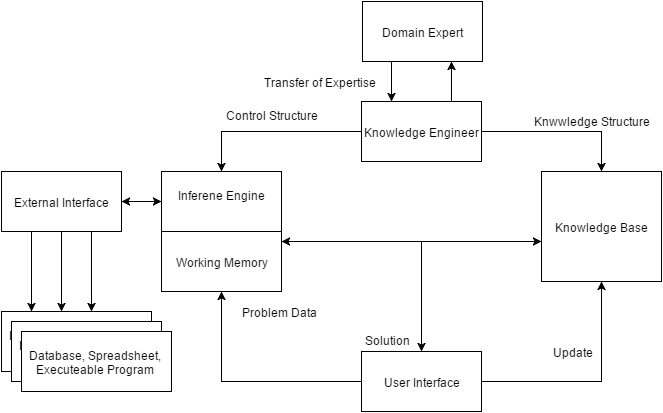
\includegraphics[scale=0.8]{gambarArsitektur.png}}\par}
	\caption{Komponen Sistem Pakar \cite{mca2015}}
	\label{fig:komponen}
\end{figure}
Penjelasan komponen penyusun dari sistem pakar sebagai berikut:

\begin{itemize}
	\item User Interface\\
	Tampilan antarmuka sebagai media komunikasi antara pengguna dengan sistem pakar.
	\item Knowledge Base\\
	Basis pengetahuan berisi pengetahuan yang relevan untuk sistem memahami, merumuskan dan memecahkan masalah. Terdiri dari dua elemen dasar yaitu fakta (facts) dan aturan (rules). Fakta menggambarkan karakteristik situasi masalah dan teori pada bidang masalah. Aturan mewakili pengetahuan ahli untuk memecahkan masalah tertentu dalam domain.
	\item Knowledge Acquisition\\
	Akuisisi pengetahuan pemecahan masalah dari pakar atau sumber pengetahuan terdokumentasi lain untuk program komputer. Potensi sumber pengetahuan bisa berupa manusia, buku teks, dokumen multimedia, database, dan laporan penelitian.
	\item Inference Engine \\
	Merupakan otak dari sistem pakar. Komponen ini menyediakan suatu metode untuk penalaran (reasoning) infromasi yang terdapat dalam knowledge base dan workplace untuk merumuskan kesimpulan.
	\item 	Workplace \\
	Sebagai tempat penyimpanan data masalah berupa hasil sementara, hipotesis dan keputusan yang sedang dikerjakan. 
	\item Explanation Subsystem \\
	Komponen tambahan yang meningkatkan kemampuan sistem pakar dengan menjelaskan kelakuan sistem pakar secara interaktif melalui jawaban pertanyaan.
	\item Knowledge Refining System \\
	Orang yang ahli di bidang tertentu dapat melakukan analisis dan peningkatan performa penafsiran miliknya. Begitu juga sistem pakar membutuhkan evaluasi untuk meningkatkan hasil yang lebih akurat melalui knowledge base serta kemampuan reasoning yang lebih efektif. 	
\end{itemize}

\section{\textit{Forward Chaining}}
Merupakan salah satu metode inferensi yang menghasilkan solusi dengan melakukan penalaran terhadap suatu masalah. Dikenal juga dengan data-driven karena inferensi dimulai dengan informasi yang tersedia kemudian baru menghasilkan konklusi. Pola pendekatan penalaran forward chaining adalah IF (informasi) THEN (konklusi). Pelacakan kedepan dilakukan dari sekumpulan fakta dan mencari kaidah yang cocok hingga menuju kesimpulan. Berikut Algoritma \ref{forwardChaining} merupakan contoh dari proses forward chaining dalam menghasilkan konklusi dari aturan produksi: 
\begin{algorithm}
	\caption{Forward chaining}
	\label{forwardChaining}
	\begin{algorithmic}[1]
		\If {$(Pasien$ $Hamil)$ AND $(kontraksi)$  AND $(premature)$}
		\State $UGD Rumah$$ Bersalin$
		\EndIf
	\end{algorithmic}
\end{algorithm}

Berikut gambar \ref{fig:inferensi} tentang ilustrasi dari proses yang terjadi pada mesin inferensi:

\begin{figure}[h]	
	{\centering {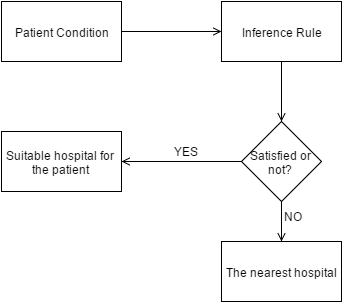
\includegraphics[scale=1]{mesinInferensi.png}}\par}
	\caption{Proses Mesin Inferensi}
	\label{fig:inferensi}
\end{figure}

Penjelasan dari proses mesin inferensi pada Gambar \ref{fig:inferensi} adalah dengan input berupa kondisi pasien. Misal pasien mengalami kelahiran premature. Dengan aturan inferensi dilakukan pengecekan dari knowledge base terhadap kecocokan rumah sakit. Mesin inferensi akan memeriksa aturan produksi terhadap UGD rumah sakit A, UGD rumah sakit B dan seterusnya. Berdasarkan kondisi pasien yang digunakan sebagai contoh maka UGD yang cocok memiliki factor waktu tempuh terdekat, terdapat dokter jaga, terdapat dokter Gynecology, tersedia ruang bersalin yang sedang kosong.

\section{Algoritma Rete}
Charles R.Forgy \cite{charles1982} mengembangkan algoritma Rete yang dikenal efisien dalam menyelesaikan berbagai permasalahan pattern matching. Merupakan solusi dari beberapa permasalahan di sistem pakar dimana jika knowledge base terdiri dari banyak rules akan menurunkan performansi. Ide utama dari algoritma rete adalah dengan melakukan komputasi himpunan rules secara instantiation incremental, berdasarkan dua pendekatan:
\begin{enumerate}
	\item Memorisation:\\ Untuk setiap siklus ke siklus selanjutnya tidak terjadi perubahan yang berarti terhadap himpunan rules. Sehingga hanya dilakukan komputasi di perubahan yang terjadi, sedangkan beberapa bagian rules tetap dipertahankan. Tidak perlu melakukan komputasi rules menyeluruh untuk tiap siklus. 
	\item Sharing:\\  Beberapa rules digunakan sebagai kondisi sama yang sering terjadi, sehingga seluruh rules difaktorkan kedalam kondisi yang terdapat mirip.
\end{enumerate}	
Implementasi algoritma Rete yaitu dengan membuat hubungan antar node yang membentuk suatu jaringan. Hubungan antar node dirancang agar bisa menghemat proses komputasi dari suatu siklus ke siklus selanjutnya. Komputasi ulang perubahan hanya untuk fakta-fakta yang akan dimodifikasi. Sebagai contoh missal diketahui sebuah rule sebagai berikut: If age fewer than 60 or age fewer than 5 or income fewer than 36000 then concession = 50/100. 
Maka jaringan Rete yang tersebut akan seperti di Gambar \ref{fig:rete} dibawah ini:
\begin{figure}[h]	
	{\centering {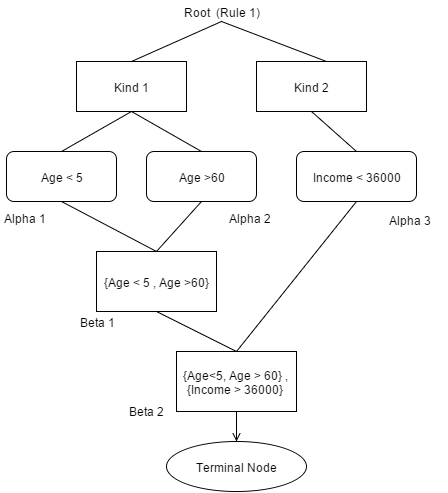
\includegraphics[scale=0.8]{jaringanRete.png}}\par}
	\caption{Contoh Jaringan terbentuk  dari algoritma Rete}
	\label{fig:rete}
\end{figure}

Penjelasan dari jaringan yang terbentuk oleh algoritma Rete pada Gambar \ref{fig:rete} adalah sebagai berikut :
\begin{enumerate}
	\item Alpha Network\\
	Berfungsi untuk memilih individu working memory element (WME) berdasarkan uji kondisional sederhana untuk membandingkan node WME yang memiliki kesamaan atribut. Percabangan mungkin terjadi pada Alpha node untuk meminimalkan redundansi.
	\item Beta Network\\
	Merupakan gabungan dari WME dan melakukan pemrosesan token. Token adalah unit penyimpanan yang berada di memori dan unit pertukaran antar memori dengan node. Setiap Beta node dapat menghasilkan token baru untuk menahan daftar WME yang merepresentasikan kecocokan partial. WME yang mencapai ujung cabang dari Beta Node merepresentasikan tahap lengkap kecocokan untuk satu produksi. Kemudian proses selanjutnya dikirim ke terminal node.
	\item Conflict Resolution\\
	Pada setiap satu siklus match-resolve-act, mesin inferensi akan menemukan semua kemungkinan kecocokan untuk fakta yang sedang diolah di working memory. Setelah semua kecocokan ditemukan, aturan produksi yang berhubungan telah diaktifkan dalam agenda. Mesin inferensi akan menentukan aturan produksi yang tereksekusi.  
\end{enumerate}
\section {SPGDT}
Sistem Penanggulangan Gawat Darurat Terpadu (SPGDT) dari dinas kesehatan merupakan sistem untuk penanggulangan pasien gawat darurat yang terdiri dari \textit{pra hospital, intra hospital} dan \textit{inter hospital} menekankan pada keselamat jiwa pasien menggunakan kode akses telekomunikasi 119\cite{kemenkes}. Layanan medis gawat darurat mengatur lebih khusus tentang penanganan medis bagi korban (standar medis Gawat Darurat, Tindakan Medis), kriteria Gawat Darurat, kriteria bukan Gawat Darurat serta pelatihan -pelatihan untuk peningkatan kompetensi SDM bidang kegawatdaruratan. \par
Informasi yang bisa didapatkan pasien melalui panggilan call center 119 adaah informasi fasilitas kesehatan dan informasi ambulan. Menggunakan \textit{call tracker} praktisi SPGDT akan menulusuri lokasi penelepon kemudian dengan algoritma kegawat daruratan yang ditetapkan oleh kementrian kesehatan terdapat alur atau langkah - langkah dalam penanganan kegawat daruratan sebagai panduan bagi agen / praktisi. Informasi ketersediaan tempat tidur sudah tersedia meliputi jumlah tempat tidur kosong di Rumah Sakit baik rawat inap maupun kamar intensif. Ketenagaan dalam bidang SPGDT meliputi :
\begin{enumerate}
	\item Koordinator
	\item Petugas Call Center 
	\item Petugas kesehatan (tenaga medis atau tenaga kesehatan lainnya)
	\item Pengemudi Ambulan
\end{enumerate}
\par
Sistem Informasi Manajemen Rumah Sakit (SIM-RS) adalah sebuah sistem informasi disiapkan untuk menangani keseluruhan proses manajemen Rumah Sakit, mulai dari pelayanan diagnosa dan tindakan pasien, rekam medis, database personalia hingga pengendalian dan manajemen kamar. SIMRS yang ideal dapat melakukan "bongkar- pasang" modul untuk bisa berkomunikasi dengan layanan lainnya diluar proses bisnis Rumah Sakit. Di Indonesia terdapat sistem informasi rawat inap yang dapat menyajikan informasi ketersedian kamar tidur rawat inap kepada pasien secara \textit{real time}. Dalam pengiriman data agar seragam dan tidak terjadi kesalahan informasi telah dibuat aturan kodefikasi oleh kementrian kesehatan dengan contoh sebagai berikut :
\begin{figure}[h]	
	{\centering {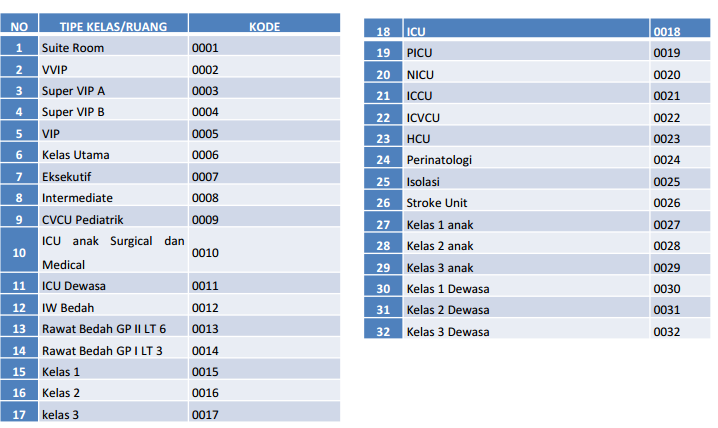
\includegraphics[scale=0.6]{kodefikasi1.png}}\par}
	\caption{Kodefikasi untuk penyeragaman kelas dan ruang RS}
	\label{fig:kodefikasi1}
\end{figure}
\par Pada Gambar \ref{fig:kodefikasi1} memperlihatkan aturan penulisan untuk ketersidaan kamar dalam Rumah Sakit, sedangkan akan diperlihatkan kodefikasi untuk tipe pasien pada gambar \ref{fig:kodefikasi2} dibawah ini :
\begin{figure}[h]	
	{\centering {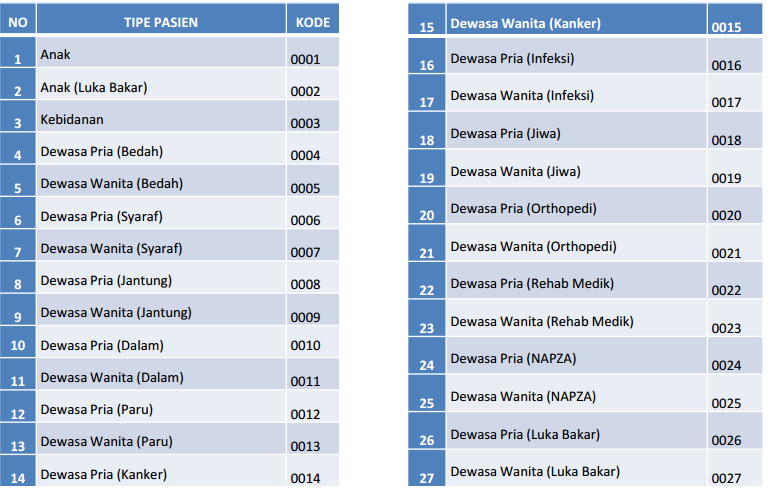
\includegraphics[scale=0.6]{kodefikasi2.png}}\par}
	\caption{Kodefikasi untuk penyeragaman tipe Pasien}
	\label{fig:kodefikasi2}
\end{figure}

\section{Kelebihan Sistem Pakar}
Pada pemrograman sistem komputer biasa yang dapat melakukan penerapan aturan bagaimana sistem atau program dapat bekerja adalah seorang ahli IT dengan menggunakan bahasa pemrogaman. Dengan dibuatnya sistem pakar aturan atau logis sistem dalam bekerja akan diterjemahkan kedalam \textit{rule} menggunakan bahasa yang mudah dipahami oleh seorang Ahli dalam ranah tertentu tidak hanya ahli IT saja. Sehingga Ahli di bidangnya dapat melakukan \textit{review} bahkan \textit{edit} terhadap aturan logis di sistem dengan pengawasan minim seorang Ahli IT atau tidak sama sekali. Dalam praktik penggunaan sistem pakar tidak menggantikan keududukan seorang pakar tetapi untuk memasyarakatkan pengetahuan dan pengalaman pakar tersebut sehingga mudah dijangkau oleh orang awam.\par
Dalam tugas akhir ini pengetahuan pakar yang akan digunakan oleh sistem adalah tenaga Ahli kegawat daruratan. Pakar ini dalam bertindak dalam ranah \textit{Pra-Hospital} untuk merujuk pasien ke Rumah Sakit yang mempunyai sumber daya sesuai kondisi pasien \cite{kemenkes}. 
\begin{figure}[h]	
	{\centering {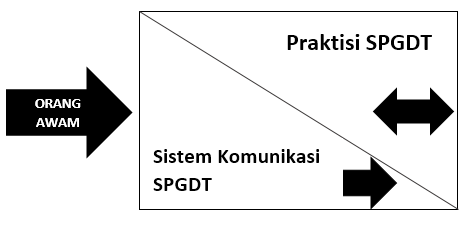
\includegraphics[scale=0.6]{praktisispgdt.png}}\par}
	\caption{Peran dan kerja praktisi SPGDT}
	\label{fig:praktisi}
\end{figure}
Dengan menggunakan sistem pakar diharapkan kerja praktisi manual seperti pada Gambar \ref{fig:praktisi} akan terbantu. Sistem yang dibangun akan meminimalisir kesalahan rujukan ke Rumah Sakit yang ternyata tidak bisa menangani pasien. Tahap program SPGDT di kota Bandung masih berjalan setengah manual (via  telepon) tetapi telihat animo masyarakat yang tinggi ditunjukkan dengan banyaknya pertanyaan yang masuk ke saluran telepon SPGDT untuk menanyakan klinik yang buka 24 jam, maupun menanyakan Rumah Sakit mana yang mempunyai kamar ICU kosong \cite{tekno}. Hasil keluaran dari sistem pakar terbukti menunjukkan keputusan yang \textit{steady, unemotional} dan \textit{complete response.}
\section{Related Works}
Penelitian terkait untuk kasus ini dilakukan Zhen \cite{zhen2014} dalam penelitiannya membangun  decision rule  untuk  penjadwalan mobil ambulans. Dalam penelitan Zhen \cite{zhen2014} memperhitungan rata-rata response time dan data stokastik kondisi lalu lintas, waktu tempuh sehingga korban gawat darurat dapat dicapai dalam waktu yang efisien. Hasilnya permintaan mobil ambulans dapat dipenuhi tepat waktu sesuai rule yang dibangun. Bowen \cite{james1998} dalam penelitiannya menggunakan sistem keputusan untuk relokasi persebaran ambulan di daerah perkotaaan dengan harapan meningkatkan kesiapan ketika terjadi kejadian gawat darurat.  Hasilnya berupa distribusi mobil ambulans yang mampu melayani permintaan di satu area secara menyeluruh. Penelitian \cite{zhen2014} dan Bowen \cite{james1998} berpusat pada bagaimana meningkatkan kinerja unit ambulan sebagai transportasi ketika terjadi kejadian gawat darurat. Namun, dalam rangka memberikan pertolongan terhadap korban gawat darurat dapat tidak hanya dibutuhkan peningkatan pelayanan mobil ambulans tetapi juga ketepatan pemilihan unit gawat darurat tujuan dengan memperhatikan sudut pandang korban dan sumber daya UGD apapun mode transportasinya.   \par
Weng dan Kuo \cite{weng2009} dalam penelitiannya membangun sistem informasi pakar gawat darurat untuk daerah dengan sumber daya medis yang kurang. Faktor yang digunakan dalma pemilihan UGD adalah kondisi pasien, jarak dari lokasi kejadian gawat darurat ke UGD tujuan,ketersediaan dokter jaga, ketersediaan ruang operasi, ketersediaan ruang ICU, ketersediaan ruang inap. Dalam penelitian tersebut dikembangkan kaidah pemilihan unit gawat darurat berdasar kondisi korban. Kaidah yang dibangun memungkinkan sistem menampilkan rumah sakit yang cocok untuk korban pada waktu kejadian gawat darurat menggunakan pola runut maju (Forward Chaining). Priyandari \cite{priyandari2011} menggunakan model kaidah pemilihan UGD dari penelitian Weng dan Kuo tetapi mengganti kriteria jarak dengan estimasi waktu tempuh untuk mengatasi arus lalulintas perkotaan yang padat. Mesin inferensi yang digunakan sama yaitu forward chaining.
\par
Dalam penelitian tugas akhir ini penulis mempertimbangkan penggunaan faktor pemilihan UGD yang dikembangkan pada penelitian Priyandari \cite{priyandari2011} dan dilakukan studi lebih lanjut model kaidah pemilihan UGD hasil dari penelitian Weng dan Kuo \cite{weng2009} untuk disesuaikan dengan studi kasus pada tugas akhir ini. Sistem yang akan dibangun berupa sistem pakar pemilihan UGD untuk wilayah kota Bandung. Algoritma yang akan diterapkan pada inference engine adalah algoritma Rete. 


%
\chapter{Analisis dan Perancangan Sistem}

\section{Gambaran Umum Sistem}
Berikut Gambar \ref{fig:GambaranUmum} merupakan diagram blok dari sistem pakar yang dibangun:

\begin{figure}[h]	
	{\centering {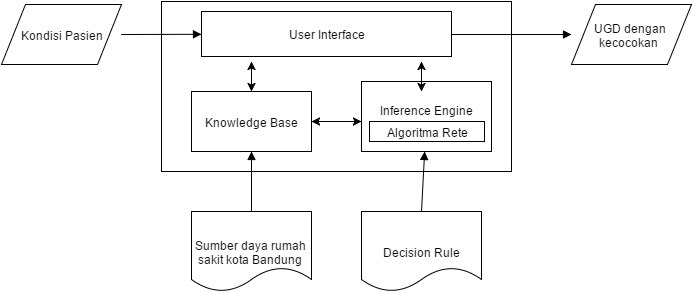
\includegraphics[scale=0.8]{gambaranUmum.png}}\par}
	\caption{Diagram Blok Gambaran Umum Sistem}
	\label{fig:GambaranUmum}
\end{figure}
Diagram blok pada Gambar \ref{fig:GambaranUmum} menggambarkan sistem dalam bekerja menerima input berupa kondisi pasien atau korban kejadian gawat darurat melalui interface sistem pakar. Knowledge base yang dibangun melalui metode pengumpulan data (observasi, wawancara pakar, studi literature) di intrepretasikan kedalam basis pengetahuan sistem pakar. Inference Engine dimana algoritma Rete diterapkan bertugas sebagai otak sistem pakar untuk melakukan pemilihan UGD berdasarkan rule dan knowledge base yang telah dibangun. \par
Berikut tahap dari pembangunan sistem pakar pemilihan UGD:
\begin{enumerate}
	\item Pembangunan knowledge base berupa informasi sumber daya rumah sakit di kota Bandung
	\item Menentukan kaidah pemilihan Unit Gawat Darurat untuk membangun decision rule yang digunakan dalam Inference Engine.
	\item Membangun inference engine dengan algoritma Rete
	\item Membangun user interface untuk menerima input berupa kondisi pasien dan menampilkan output berupa UGD dengan kecocokan yang dihasilkan oleh Inference Engine.
\end{enumerate} 
\par
Berikut simulasi menggambarkan bagaimana sistem yang dibangun bekerja akan diperlihatkan : 

\begin{figure}[h]	
	{\centering {\includegraphics[scale=0.9]{captureSimulasi.png}}\par}
	\caption{Simulasi sistem}
	\label{fig:simulasi}
\end{figure}
\par
Selanjutnya sistem akan memberikan lokasi dari Rumah Sakit yang merupakan keluaran dari sistem pakar, pada kasus ini adalah lokasi Rumah Bersalin Tunas Harapan yang diperlihatkan pada Gambar \ref{fig:hasil}. 
\begin{figure}[h]	
	{\centering \frame{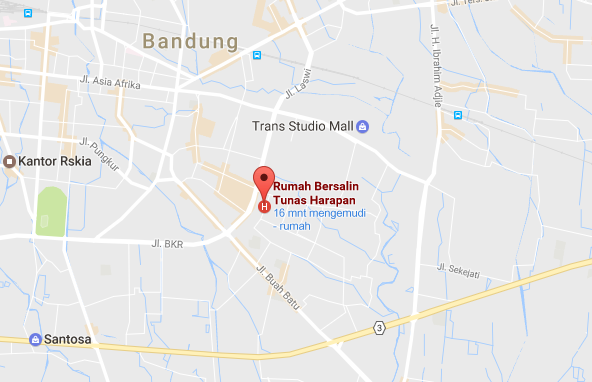
\includegraphics[scale=0.5]{hasilSistem.png}}\par}
	\caption{Lokasi RS UGD hasil keluaran sistem}
	\label{fig:hasil}
\end{figure}

\section{Data Kriteria}
Data kriteria pada tugas akhir ini merupakan data apa saja yang dijadikan pertimbangan dalam pemilihan Unit Gawat Darurat dalam suatu Rumah Sakit. Berdasarkan penelitian sebelumnya Weng dan Kuo \cite{weng2009} menggunakan kriteria ketersediaan dokter jaga, dokter bedah, dokter spesialis, ketersediaan ruang operasi dan kamar inap dan Jarak antara pasien dan lokasi UGD. Sedangkan Priyandari \cite{priyandari2011} melakukan perbaikan dengan mengganti jarak UGD menjadi waktu tempuh untuk menuju UGD. \par
Berdasarkan peraturan Kementrian Kesehatan RI \cite{kemenkes} dalam SPGDT (Sistem Penanggulangan Gawat Darurat Terpadu) telah diatur informasi data yang harus dikeluarkan oleh Rumah Sakit di Indonesia. Seperti data informasi fasilitas kesehatan terdekat, data informasi ketersediaan tempat tidur, ketersediaan Dokter, dll. Telah dilakukan penyeragaman kamus data antar Rumah Sakit sehingga dapat terhubung antar satu dan lainnya. Berikut Gambar \ref{fig:dataRS} adalah contoh data yang dikeluarkan oleh SPGDT:
\begin{figure}[h]	
	{\centering \frame{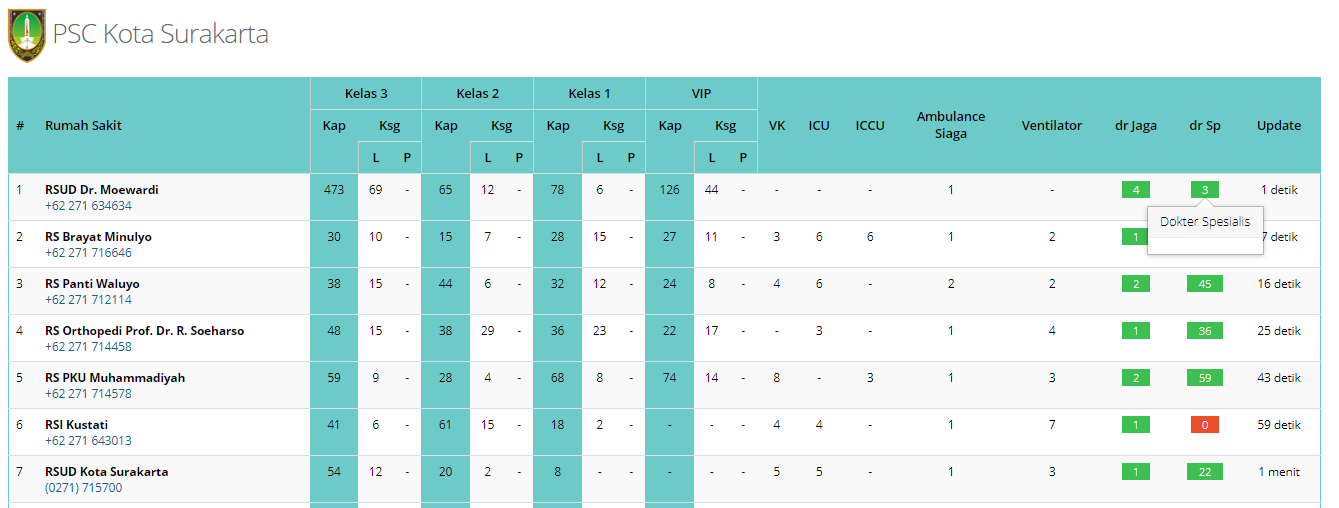
\includegraphics[scale=0.4]{dataRS.png}}\par}
	\caption{Data ketersediaan Rumah Sakit dari SPGDT}
	\label{fig:dataRS}
\end{figure}
\par
Keterangan untuk Gambar \ref{fig:dataRS}:
\begin{enumerate}
	\item Kap 	: Kapasitas 
	\item Ksg	: Kosong L/P
	\item VK		: Verlos Karmer (Ruang Bersalin)
	\item ICU	:  Intensif Care Unit
	\item ICCU	:  Intensif Cardiology Care Unit (Jantung)
	\item dr Jaga	: Doktek Jaga
	\item dr SP	: Dokter Spesialis
\end{enumerate}
\par
Dari data ketersedian fasilitas Rumah Sakit diatas system pakar yang dibangun diaharapkan dapat memilihkan UGD yang tepat sesuai kondisi pasien. Untuk data ketersedian Dokter jaga dan Dokter spesialis tersedia dalam SPGDT seperti terlihat dalam Gambar \ref{fig:dataDok} berikut :

\begin{figure}[h]	
	{\centering \frame{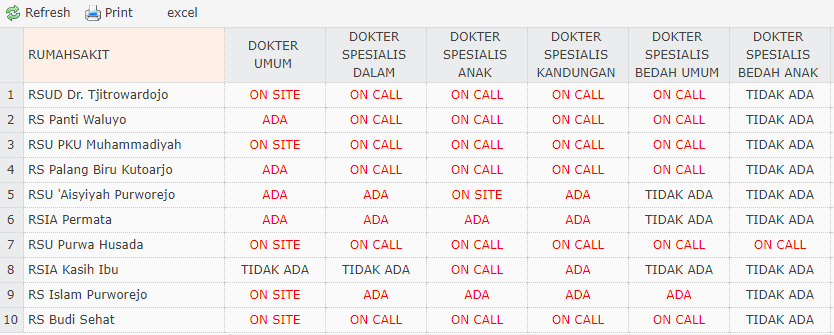
\includegraphics[scale=0.6]{dataDokter.png}}\par}
	\caption{Data ketersediaan Dokter Rumah Sakit dari SPGDT}
	\label{fig:dataDok}
\end{figure}

\par Dalam tugas akhir kriteria yang akan digunakan adalah ketersediaan ruang rawat inap ICU, ICCU, ruang operasi atau kamar bersalin. ketersediaan Dokter Spesialis, Kriteria kejadian berupa lokasi kejadiaan atau pasien dimana akan digunakan untuk menghitung waktu tempuh ke UGD. Untuk waktu tempuh didapat menggunakan Google Maps API V2.

\section{Uji Akurasi}
Hasil yang didapat berupa UGD yang terpilih oleh inference engine sesuai knowledge dan decision rule berdasarkan input kondisi pasien akan dibandingkan dengan pilihan dari pakar tenaga medis untuk mengetahui nilai akurasi sistem pakar pemilihan UGD yang dibangun dalam tugas akhir ini.

\section{Fungsional Sistem}
Fungsional sistem yang akan dibangun ini antara lain adalah :
\begin{enumerate}
	\item Sistem dapat menerima Input berupa kondisi calon pasien serta data kertersediaan Rumah Sakit
	\item Sistem dapat menampilkan lokasi UGD Rumah Sakit hasil keluaran sistem pakar
	\item Sistem dapat menerima inputan perbaikan aturan produksi sistem pakar dari user ahli
	\item Sistem menampilkan panduan pengguna, syarat dan ketentuan pemakaian
\end{enumerate}

\section{Deskripsi Lingkup Operasional}
Dalam penelitian ini, lingkup operasional yang digunakan baik itu perangkat
keras maupun perangkat lunak dijelaskan sebagai berikut:
\begin{enumerate}
	\item Spesifikasi Perangkat Keras\\
	Perangkat keras yang digunakan pada penelitian ini memiliki spesifikasi sebagai berikut :
	\begin{enumerate}
		\item Notebook Acer Aspire E5-553G-11Q
		\item AMD Quad-Core Processor A12-9700P 3.40 Ghz
		\item 8GB DDR4 Memory
		\item Radeon R8 M445DX 2GB
	\end{enumerate}
	\item Spesifikasi Perangkat Lunak\\
	Perangkat lunak yang digunakan pada penelitian ini memiliki spesifikasi sebagai berikut :
		\begin{enumerate}
		\item Sistem Operasi Windows 10 Pro 64bit
		\item Sublime Text Editor
		\item Google Maps API V2
		\item Git version control
	\end{enumerate}
\end{enumerate}

%
\chapter{Analisis dan Perancangan Sistem}
\section{title}

tulis analisis dan perancangan

\section{Persamaan Air Dangkal}
Berikut diberikan persamaan pengatur dari persamaan gelombang pada gitar
\begin{equation}\label{nama-rumus}
\int_0^1 \frac{f(x)}{g(x)}\ {\rm dx}=\sin x
\end{equation}

Rumus (\ref{nama-rumus}) merupakan contoh persamaan matematika. persamaan matematika diatas diberi nama \textbackslash label\{nama-rumus\}.

\begin{figure}[h!]
	\centering
	% 
\includegraphics[scale=0.3]{Tel-U-Logo.png}
	\caption{Caption}
	\label{fig:my_label}
\end{figure}
\subsection{Cara memanggil pustaka}

%
%\include{Kesimpulan}
%
\cleardoublepage
\addcontentsline{toc}{chapter}{Daftar Pustaka}
\bibliographystyle{acm} %harvard style
\bibliography{References}
%
%\pagebreak
\cleardoublepage
\addcontentsline{toc}{chapter}{Lampiran}
\chapter*{Lampiran}

\end{document}
